\input{preamble-report}

\title{\textbf{Uncertainty Budget for Phase-Shifting Fizeau Interferometry of Optical Flats}\\[0.6em]
\large Demonstration scientific engineering report}
\author{\docowner}
\date{15~November~2026}

\begin{document}
\maketitle

\begin{tcolorbox}[colback=black!4, colframe=black, boxrule=0.6pt]
\textbf{Demonstration project.} The instrument, laboratory, and numerical example are fictional. Equations, standards, and cited publications are real. This report is not a commercial study and is not affiliated with any manufacturer.
\end{tcolorbox}

\begin{abstract}
\noindent
A combined standard uncertainty is derived for the peak-to-valley surface form of a \SI{100}{\milli\meter} optical flat measured in a laser Fizeau interferometer. Starting from the optical path difference of a double-pass cavity and a five-bucket phase-shifting algorithm, the report converts wrapped phase to surface height and assigns Type~A and Type~B terms following JCGM~100:2008. For the demonstration configuration, the dominant contributions are the uncalibrated transmission-flat residual, focus-induced edge diffraction, and cavity air-index drift. The combined standard uncertainty over a \SI{90}{\milli\meter} clear aperture is \(u_c(\PV)=\SI{3.4}{\nano\meter}\) (\(k=1\)).
\end{abstract}

\section{Introduction}

Optical drawings specify surface form in the language of ISO~10110-5 \cite{iso10110-5}. Interpreting a Fizeau measurement against that specification requires more than a single \(\PV\) number: the interferometer, the transmission reference, the environment, and the analysis aperture all contribute \cite{iso14999-4,malacara2007}. This report constructs an uncertainty budget for one well-defined case---a plane test surface measured against a transmission flat at \wavelength---so that a documentation set can point to a traceable numerical argument rather than to an unexplained software statistic.

The demonstration instrument is the fictional \instrumentlong\ described in the companion operating manual. The numerical values in Table~\ref{tab:budget} are internally consistent example data, not laboratory results.

\section{Measurement model}

\subsection{Optical path difference}

In a Fizeau cavity the test and reference beams share the instrument optics. The optical path difference at each pixel is \cite{bornwolf1999,malacara2007}
\begin{equation}
  \OPD(x,y) = 2\,n\,h(x,y) + \OPD_{\mathrm{ref}}(x,y) + \varepsilon_{\mathrm{retrace}}(x,y),
  \label{eq:opd}
\end{equation}
where \(h\) is the test-surface height relative to the transmission-flat vertex plane, \(n\) is the refractive index of the cavity air, \(\OPD_{\mathrm{ref}}\) is residual reference-surface error, and \(\varepsilon_{\mathrm{retrace}}\) collects off-axis pupil errors that appear when the return beam does not retrace the instrument axis.

\subsection{Phase-shifting equation}

A temporal phase-shifting acquisition records intensities
\begin{equation}
  I_k = I' + I''\cos(\phase + \delta_k), \qquad k = 0,\ldots,4,
  \label{eq:Ik}
\end{equation}
with nominal shifts \(\delta_k = k\pi/2\). The Schwider--Hariharan five-bucket estimator \cite{schwider1983,hariharan1987,creath1988} is
\begin{equation}
  \phase = \operatorname{atan2}\bigl(2I_1 - 2I_3,\; I_0 - 2I_2 + I_4\bigr).
  \label{eq:phase}
\end{equation}
Wrapped phase is related to optical path by \(\phase = (2\pi/\lambda)\,\OPD\). Solving Eq.~\eqref{eq:opd} for height, with \(n\approx 1\) and \(\OPD_{\mathrm{ref}}\) subtracted when a calibration map exists,
\begin{equation}
  h(x,y) = \frac{\lambda}{4\pi}\,[\phase(x,y)-\phase_{\mathrm{ref}}(x,y)] - \tfrac12\varepsilon_{\mathrm{retrace}}(x,y).
  \label{eq:height}
\end{equation}
Surface \(\PV\) over a clear aperture \(\mathcal{A}\) is
\begin{equation}
  \PV = \max_{\mathcal{A}} h - \min_{\mathcal{A}} h
  \label{eq:pv}
\end{equation}
after removal of piston and tilt, which is the ISO~10110-5 default reduction for a flat \cite{iso10110-5,bruning1974,wyant2013}.

\subsection{Air index}

A small temperature change \(\Delta T\) in the cavity changes \(n\) and therefore the reported height scale. Using a simplified Edl\'en dependence, \(\partial n/\partial T \approx \SI{-9e-7}{\per\celsius}\) near \SI{20}{\celsius}. For a cavity length \(L\), a uniform index change is largely common-mode in a Fizeau geometry; the residual that survives is the \emph{gradient} across the aperture, treated here as a Type~B slope uncertainty \(u_n\).

\section{Uncertainty contributions}

Terms are evaluated as standard uncertainties (\(k=1\)) at the reported \(\PV\) of the test flat, \(\CA=\SI{90}{\milli\meter}\). Type~A terms come from repeatability of the demonstration data set (\(N=12\) repeats without remounting, and \(N=6\) with remounting). Type~B terms are rectangular distributions converted with \(u = a/\sqrt{3}\) unless noted \cite{jcgm100}.

\begin{table}[ht]
\centering
\caption{Uncertainty budget for \(\PV\) surface form. Values are demonstration data for \instrument.}
\label{tab:budget}
\begin{tabular}{@{}l l c c c@{}}
\toprule
Symbol & Contribution & Type & \(u_i\) (\nm) & Sensitive to \\
\midrule
\(u_{\mathrm{A,rep}}\) & Repeatability, no remount & A & 0.6 & turbulence, camera noise \\
\(u_{\mathrm{A,mount}}\) & Remounting the test flat & A & 1.1 & fixture, alignment \\
\(u_{\mathrm{TF}}\) & Transmission-flat residual after subtraction & B & 2.4 & calibration artefact \\
\(u_{\mathrm{focus}}\) & Residual edge diffraction after focus & B & 1.5 & imaging NA, part diameter \\
\(u_{\delta}\) & Phase-shifter miscalibration & B & 0.4 & \(\delta_k\) error \\
\(u_{n}\) & Air-index gradient & B & 0.7 & \(\Delta T\), cavity length \\
\(u_{\mathrm{retrace}}\) & Off-axis retrace & B & 0.8 & \TF\ tilt, zoom \\
\(u_{\mathrm{scale}}\) & Pixel-scale and aperture definition & B & 0.5 & \(\CA\) mask \\
\bottomrule
\end{tabular}
\end{table}

Assuming uncorrelated contributors \cite{jcgm100},
\begin{equation}
  u_c^2(\PV) = \sum_i u_i^2.
  \label{eq:uc}
\end{equation}
Substitution of Table~\ref{tab:budget} yields
\begin{equation}
  u_c(\PV) = \SI{3.4}{\nano\meter} \quad (k=1).
  \label{eq:ucnum}
\end{equation}
An expanded uncertainty \(U = k\,u_c\) with \(k=2\) is \(\SI{6.8}{\nano\meter}\), or \(\waves{0.011}\) at \wavelength. This example does \emph{not} claim a product specification; it shows the arithmetic a production quality system would attach to a report.

\begin{figure}[ht]
\centering
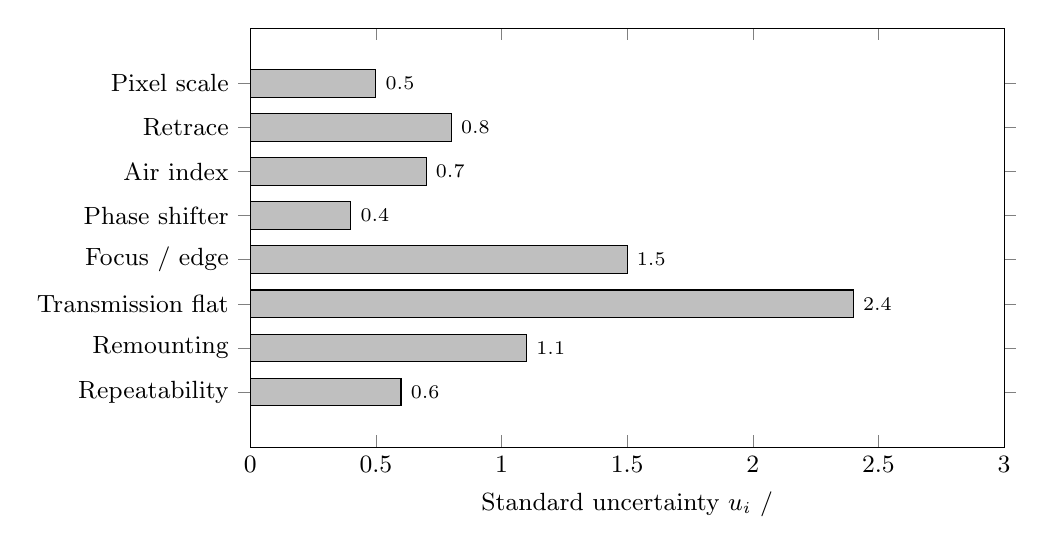
\begin{tikzpicture}
\begin{axis}[
  xbar,
  width=0.92\textwidth,
  height=7.2cm,
  xlabel={Standard uncertainty \(u_i\) / \si{\nano\meter}},
  symbolic y coords={
    Repeatability,
    Remounting,
    Transmission flat,
    Focus / edge,
    Phase shifter,
    Air index,
    Retrace,
    Pixel scale},
  ytick=data,
  nodes near coords,
  nodes near coords align={horizontal},
  every node near coord/.append style={font=\scriptsize},
  xmin=0, xmax=3.0,
  y=5.6mm,
  enlarge y limits={abs=7mm},
  tick label style={font=\small},
  label style={font=\small}
]
\addplot[fill=black!25] coordinates {
  (0.6,Repeatability)
  (1.1,Remounting)
  (2.4,Transmission flat)
  (1.5,Focus / edge)
  (0.4,Phase shifter)
  (0.7,Air index)
  (0.8,Retrace)
  (0.5,Pixel scale)
};
\end{axis}
\end{tikzpicture}
\caption{Relative size of the standard-uncertainty terms in Table~\ref{tab:budget}. The transmission-flat residual dominates unless a better artefact or a two-flat test is used.}
\label{fig:bars}
\end{figure}

\section{Notes on selected terms}

\paragraph{Transmission flat.}
Without subtraction, a \(\lambda/20\) \(\PV\) reference would contribute \(\SI{31.6}{\nano\meter}\) and would dwarf every other term. The \(\SI{2.4}{\nano\meter}\) entry assumes a stored calibration map whose own uncertainty is that of the artefact plus the transfer measurement \cite{malacara2007}.

\paragraph{Focus.}
An out-of-focus Fizeau image produces a characteristic rolled edge from diffraction at the part boundary. The operating-manual focus procedure (rough visual focus, then jog on the measured edge zone) is the control for \(u_{\mathrm{focus}}\). Eroding edge pixels after a poor focus hides the symptom and biases \(\CA\); it is not a substitute for the procedure.

\paragraph{Phase shifter.}
The five-bucket algorithm is first-order insensitive to a linear calibration error in \(\delta_k\) \cite{hariharan1987,creath1988}. The remaining Type~B assignment is a bound on second-order residuals from the instrument's phase-shifter check.

\section{Reporting}

A measurement report consistent with this budget should state, at minimum:

\begin{itemize}
  \item instrument and transmission-flat identifications
  \item wavelength and analysis terms removed (piston and tilt)
  \item clear aperture and pixel scale
  \item whether reference subtraction was active
  \item \(\PV\), \(\RMS\), and \(U(k=2)\) on the same aperture
\end{itemize}

ISO~14999-4 discusses how those reported values relate to a drawing tolerance \cite{iso14999-4}. This demonstration stops at \(u_c\); a production laboratory would add the decision rule used to accept or reject the part.

\section{Conclusion}

For the fictional \instrument\ measuring a \SI{100}{\milli\meter} flat, a GUM combination of the Table~\ref{tab:budget} terms gives \(u_c(\PV)=\SI{3.4}{\nano\meter}\). The budget is dominated by the working reference, then by focus and remounting. Those three terms are also the ones an operating manual can actually control: artefact quality, a deterministic focus procedure, and a repeatable mount. Custom LaTeX commands for \(\PV\), \(\RMS\), \(\OPD\), and SI units are shared with the companion manual so the two documents do not drift apart in notation.

\printbibliography

\end{document}
